% Created 2021-01-20 Wed 13:55
% Intended LaTeX compiler: pdflatex
\documentclass[unicode, 12pt, xdvipdfmx, aspectratio=43]{beamer}
\usepackage[utf8]{inputenc}
\usepackage[T1]{fontenc}
\usepackage{graphicx}
\usepackage{grffile}
\usepackage{longtable}
\usepackage{wrapfig}
\usepackage{rotating}
\usepackage[normalem]{ulem}
\usepackage{amsmath}
\usepackage{textcomp}
\usepackage{amssymb}
\usepackage{capt-of}
\usepackage{hyperref}
\usepackage[backend=bibtex, style=authoryear, maxcitenames=2]{biblatex}
\addbibresource{../resources/anthology.bib}
\addbibresource{../resources/my.bib}
\let\oldcite\cite
\renewcommand{\cite}[1]{{\scriptsize\reffont{(\oldcite{#1})}}}
\newcommand{\citet}[2][\footnotesize]{{\reffont#1\citeauthor*{#2} (\citeyear{#2})}}
\newcommand{\mycite}[1]{{\scriptsize\reffont({\citeauthor*{#1}, \citeyear{#1}})}}
\newcommand{\myfootcite}[1]{\footnote{\tiny\reffont\citetitle{#1}, \citeauthor*{#1}, \citeyear{#1}.}}
\usepackage{hyperref}
\usetheme{metropolis}
\setbeamertemplate{items}[default]
\setbeamertemplate{itemize item}{\small\raise0.5pt\hbox{$\blacksquare$}}
\setbeamertemplate{itemize subitem}{\footnotesize\raise1.5pt\hbox{$\bullet$}}
\setbeamertemplate{itemize subsubitem}{\scriptsize\raise1.5pt\hbox{$\blacktriangleright$}}
\setbeamertemplate{enumerate item}{\textbf{(\arabic{enumi})}}
\addtolength{\skip\footins}{6pc plus 10pt}
\usepackage{xltxtra}
\usepackage{booktabs}
\usepackage[absolute,overlay]{textpos}
\usepackage{pgfpages}
\usepackage{tikz}
\usepackage{tikz-dependency}
\usetikzlibrary{arrows.meta, matrix, positioning, fit, calc, backgrounds, shapes.callouts}
\usepackage{pgfgantt}
\usepackage{adjustbox}
\usepackage{array}
\usepackage[linguistics]{forest}
\newcommand{\highlightcap}[3][blue]{\tikz[baseline=(x.base)]{\node[rectangle,rounded corners,fill=#1!20](x){#2} node[below=0.5ex of x, color=#1]{#3};}}
\newcommand{\highlight}[2][blue]{\tikz[baseline=(x.base)]{\node[rectangle,rounded corners,fill=#1!20](x){#2};}}
\newcommand{\calloutbase}[2]{\tikz[remember picture, baseline=(#1.base)]{\node(#1) {#2};}}
\newcommand{\calloutpos}[2]{\tikz[remember picture, overlay]{\node[below=0cm of #1] {#2};}}
\newcommand{\calloutbelow}[3][blue]{\tikz[remember picture, overlay]{\node[rectangle callout, rounded corners, fill=#1!10, callout absolute pointer={(#2.south)}, below=of #2] {#3};}}
\usepackage{xcolor}
\definecolor{myalert}{HTML}{AD003D}
\definecolor{mDarkTeal}{HTML}{23373b}
\definecolor{mLightGreen}{HTML}{14B03D}
\usefonttheme{professionalfonts}
\usepackage[T1]{fontenc}
\usepackage{fontspec}
\XeTeXlinebreaklocale "ja"
\usepackage{xeCJK}
\setsansfont[BoldFont={Fira Sans Bold}]{Fira Sans Book}
\setCJKmainfont{Noto Sans CJK JP}
\setCJKsansfont{Noto Sans CJK JP}
\setCJKromanfont{Noto Serif CJK JP}
\xeCJKDeclareCharClass{CJK}{`※}
\newfontfamily\firasans{Fira Sans}
\newfontfamily\emojifont{Noto Emoji}
\newfontfamily\octicons{github-octicons}
\newfontfamily\materials{Material Icons}
\newfontfamily\faicons{FontAwesome}
\newfontfamily\reffont{Times New Roman}
\usepackage{amssymb}
\usepackage{mathfont}
\usepackage{bbm}
\newcommand{\argmax}{\mathop{\rm arg~max}\limits}
\newcommand{\argmin}{\mathop{\rm arg~min}\limits}
\renewcommand{\baselinestretch}{1.3}
\usetheme{default}
\author{出口 ~ 祥之 \\ \lower2.0pt\hbox{\materials} \texttt{deguchi@ai.cs.ehime-u.ac.jp}}
\date{2021/01/20 ~ 二宮研 論文輪読会}
\title{Fully Non-autoregressive \\ Neural Machine Translation: \\ Tricks of the Trade}
\subtitle{(Jiatao Gu and Xiang Kong, 2020)}
\institute{}
\hypersetup{
 pdfauthor={出口 ~ 祥之 \\ \lower2.0pt\hbox{\materials} \texttt{deguchi@ai.cs.ehime-u.ac.jp}},
 pdftitle={Fully Non-autoregressive \\ Neural Machine Translation: \\ Tricks of the Trade},
 pdfkeywords={},
 pdfsubject={},
 pdfcreator={Emacs 27.1 (Org mode 9.3)}, 
 pdflang={English}}
\begin{document}

\maketitle

\begin{frame}[label={sec:orgb065a1d}]{\hbox{\octicons} Links}
\begin{block}{\raise0.5pt\hbox{\octicons} Paper}
\begin{block}{\url{https://arxiv.org/abs/2012.15833}}
\end{block}
\end{block}
\end{frame}
\begin{frame}[label={sec:org8e2dbed}]{Introduction}
\begin{block}{NAT が Autoregressive Transformer と comparable に}
\begin{itemize}
\item WMT14 En-De: 27.49 BLEU (\%),翻訳速度 16.5x
\begin{itemize}
\item Autoregressive Transformer から性能を劣化させずに翻訳速度を改善
\end{itemize}
\end{itemize}

\begin{center}
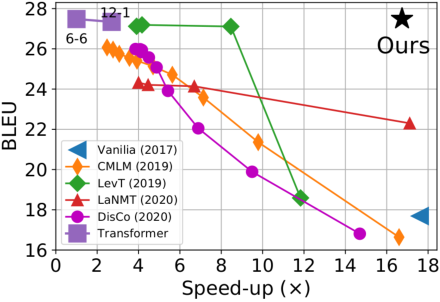
\includegraphics[width=0.6\linewidth]{./figure/Figure1.pdf}
\end{center}
\end{block}
\end{frame}

\begin{frame}[label={sec:org90405f0}]{Motivation}
\begin{block}{NAT とは何か,なぜ性能が劣化しやすいか}
\begin{itemize}
\item AT と NAT の比較
\end{itemize}
\centering
\begin{tabular}{lcc} \toprule
  & AT & NAT \\\midrule
生成確率 & $p_\theta(y_t |  y_{<t}, x_{1:T'})$ & $\prod_{t=1}^T p_\theta(y_t  | x_{1:T'})$ \\
生成時間 & $O(T)$ & $O(1)$ \\
\bottomrule
\end{tabular}

\begin{itemize}
\item \small NAT の問題点: 目的言語文中の単語共起を捉えられない
\begin{center}
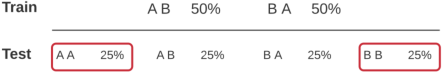
\includegraphics[width=0.7\linewidth]{./figure/Figure2.pdf}
\end{center}

\begin{itemize}
\item 解決策?: Iterative refinement (← non ``fully-NAT''\ldots{})
\end{itemize}
\end{itemize}
\end{block}
\end{frame}

\begin{frame}[label={sec:org69365c3}]{Proposed Method}
\begin{block}{single forward で生成できる ``fully-NAT''}
\begin{itemize}
\item 従来研究で提案されてきた数々の NAT モデルは出力単語間の \textbf{\alert{依存削減 (dependency reduction)}} を目的として設計
\begin{itemize}
\item cf. 数々の NAT モデル: \\
\scriptsize \url{https://github.com/kahne/NonAutoregGenProgress}
\end{itemize}
\item 複数の手法を組み合わせて\alert{依存削減}することにより,fully-NAT で AT の性能に追い付く
\end{itemize}
\end{block}
\end{frame}

\begin{frame}[label={sec:org53115a7}]{Data: Knowledge Distillation (KD)}
\begin{block}{訓練データの目的言語文を教師モデルの出力に置換}
\begin{itemize}
\item 最も効果の高い依存削減
\item 目的言語文のノイズが減る
\item 原言語文との対応関係がより決定的に
\item 教師モデルのサイズは NAT モデルに応じて適切に選ぶ必要がある
\end{itemize}

\metroset{block=fill}
\begin{block}{NAT と KD についての解析 (ICLR 2020):}
\scriptsize \url{https://jiataogu.me/publication/understand-distillation}
\end{block}
\end{block}
\end{frame}

\begin{frame}[label={sec:org1345e82}]{Model: Latent Variables}
\begin{block}{\citet[\normalsize]{shu-etal-2020-latent} のモデルを採用}
\vspace{-0.4cm}
\begin{center}
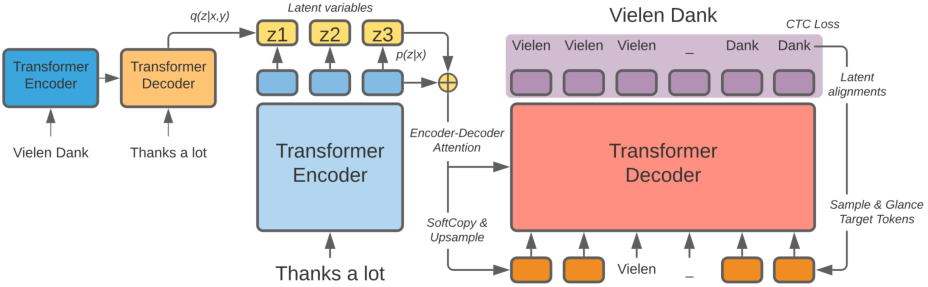
\includegraphics[width=0.85\linewidth]{./figure/Figure3.pdf}
\end{center}

\begin{columns}
\begin{column}{1.1\columnwidth}
\vspace{-0.5cm}
\begin{description}
\item[{生成確率:}] \(p_\theta (\boldsymbol{y}|\boldsymbol{x}) = \int_{\boldsymbol{z}} p_\theta (\boldsymbol{z}|\boldsymbol{x}) \prod_{t=1}^T p_\theta (y_t | \boldsymbol{z}, \boldsymbol{x}) d\boldsymbol{z}\)
\item[{ELBO:}] \(\underbrace{\mathbb{E}_{\boldsymbol{z} \sim q_\phi} \left[ \log p_\theta (\boldsymbol{y} | \boldsymbol{z}, \boldsymbol{x}) \right]}_{\text{likelihood}} - \mathcal{D}_{\mathrm{KL}} (q_\phi (\boldsymbol{z} | \boldsymbol{x}, \boldsymbol{y} ) \parallel p_\theta ( \boldsymbol{z} | \boldsymbol{x}))\)
\end{description}
\end{column}
\end{columns}

\begin{block}{}
\vspace{-0.7cm}
\begin{itemize}
\item 事後確率 \(q_\phi (\boldsymbol{z} | \boldsymbol{x}, \boldsymbol{y} )\) を得るために Encoder-Decoder モデルを使用
\item \(\theta\) と \(\phi\) の間で embedding layer のみパラメータ共有
\end{itemize}
\end{block}
\end{block}
\end{frame}

\begin{frame}[label={sec:orgc26c53b}]{Loss Function: Latent Alignments}
\begin{block}{cross entropy (CE) loss の代わりに CTC loss を採用}
\begin{center}
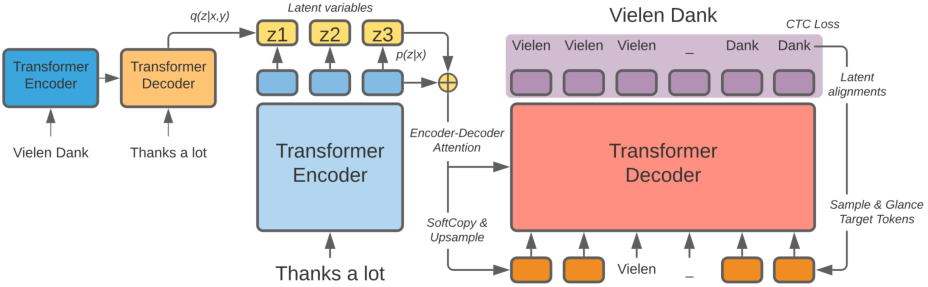
\includegraphics[width=\linewidth]{./figure/Figure3.pdf}
\end{center}

\begin{itemize}
\item CE: 出力の位置のずれに対して敏感
\item CTC: 出力位置に柔軟性をもたせる \cite{saharia-etal-2020-nonautoregressive}
\vspace{-0.3cm}
\begin{equation*}
  \log p_\theta (\boldsymbol{y}|\boldsymbol{x}) = \log \sum_{\boldsymbol{a}\in\Gamma(\boldsymbol{y})} p_\theta (\boldsymbol{a}|\boldsymbol{x}), ~ \boldsymbol{a}: \text{latent alignments}
\end{equation*}
\end{itemize}

\begin{textblock*}{\linewidth}(195pt, 82pt)
  \begin{adjustbox}{width=0.35\linewidth}
    \tikz{\draw[rounded corners, line width=3pt, green] (0, 0) rectangle (5.5, 1);}
  \end{adjustbox}
\end{textblock*}
\end{block}
\end{frame}

\begin{frame}[label={sec:org2fcf98a}]{Learning: Glancing Targets}
\begin{block}{訓練時に目的言語文をランダムにマスクして入力 \cite{ghazvininejad-etal-2019-mask}}
\begin{itemize}
\item 訓練時の目的関数: \\
\(\log p_\theta (\boldsymbol{y} | \boldsymbol{x})\) → \(\log p_\theta (\boldsymbol{y} | \boldsymbol{m} \odot \boldsymbol{y}, \boldsymbol{x}), \boldsymbol{m} \sim \gamma (l, \boldsymbol{y}), l \sim \mathcal{U}_{|\boldsymbol{y}|}\) \\
\begin{itemize}
\item \(\boldsymbol{m}\) : マスク
\item \(\gamma\) : マスクトークン数 \(l\) を受け取るサンプル関数
\end{itemize}

\item カリキュラム学習によって訓練 (GLAT) \cite{qian-etal-2020-glancing}
\begin{itemize}
\item 訓練時と翻訳時のギャップを埋める
\item \(l \sim g(f_{ratio} \cdot \mathcal{D}(\hat{\boldsymbol{y}}, \boldsymbol{y}))\) 
\begin{itemize}
\item \(\mathcal{D}\) はモデル予測 \(\hat{\boldsymbol{y}}\) と正解との差 (レーベンシュタイン距離など)
\item \(f_{ratio}\) はマスク割合 (ハイパーパラメータ)
\item 本論文では \(g\) にポアソン分布を使用
\end{itemize}
\end{itemize}
\end{itemize}
\end{block}
\end{frame}

\begin{frame}[label={sec:org55d02f3}]{Learning: Glancing Targets}
\begin{itemize}
\item 訓練時のデコーダ入力長
\begin{itemize}
\item GLAT \cite{qian-etal-2020-glancing} : 参照訳のトークン長
\item 提案モデル (CTC-based) : 出力系列長 \(\ge\) 入力系列長
\begin{itemize}
\item viterbi aligned tokens: \(\hat{\boldsymbol{a}} = \argmax_{\boldsymbol{a} \in \Gamma (\boldsymbol{y})} p_\theta (\boldsymbol{a} | \boldsymbol{x})\)
\end{itemize}
\end{itemize}
\end{itemize}
\end{frame}

\begin{frame}[label={sec:orgdb5043c}]{Summary}
\begin{columns}
\begin{column}{1.15\columnwidth}
\begin{center}
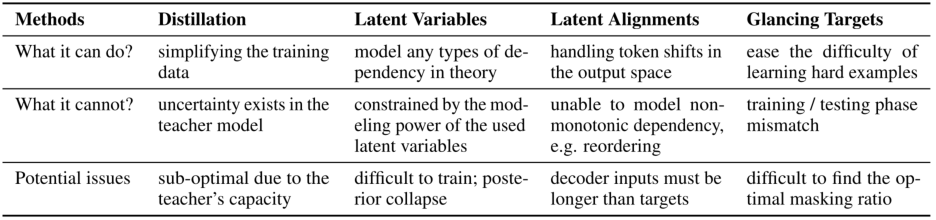
\includegraphics[width=\linewidth]{./figure/Table1.pdf}
\end{center}
\end{column}
\end{columns}
\end{frame}

\begin{frame}[label={sec:orgc35dc6f}]{Experiments}
\begin{block}{Dataset}
\begin{itemize}
\item WMT14 EN \(\leftrightarrow\) DE (4.0M)
\item WMT16 EN \(\leftrightarrow\) RO (610k)
\item WMT20 JA \(\rightarrow\) EN (13M (filterd))
\end{itemize}
\end{block}

\begin{block}{Knowledge Distillation}
\begin{itemize}
\item 教師モデルによって生成した目的言語文から学習
\begin{itemize}
\item WMT14 EN \(\leftrightarrow\) DE, WMT16 EN \(\leftrightarrow\) RO: Transformer \textit{base}
\item WMT20 JA \(\rightarrow\) EN: Transformer \textit{big}
\end{itemize}
\item ビーム幅 5 のビーム探索で目的言語文を生成
\end{itemize}
\end{block}
\end{frame}

\begin{frame}[label={sec:orge88ef1e}]{Experiments}
\begin{block}{Decoding}
\begin{itemize}
\item 各位置で最大確率を持つトークンを生成後, \(\Gamma^{-1}\) によって出力を獲得
\item noisy parallel decoding (NPD) \cite{gu-etal-2018-non}
\item ビーム探索や \(n\text{-gram}\) 言語モデルと組み合わせ
\vspace{-0.3cm}
\begin{equation*}
  \log p_\theta (\boldsymbol{y} | \boldsymbol{x}) + \alpha \log p_{\mathrm{LM}} (\boldsymbol{y}) + \beta \log |\boldsymbol{y}|
\end{equation*}
\end{itemize}
\end{block}

\begin{block}{Baselines: Autoregressive Transformer (AT)}
\begin{itemize}
\item \textit{base}
\item \textit{big}
\item \textit{Deep Encoder-Shallow Decoder} (12-1) \cite{kasai-etal-2021-deep}
\end{itemize}
\end{block}
\end{frame}

\begin{frame}[label={sec:orgc5defef}]{Evaluation}
\begin{description}
\item[{翻訳性能}] BLEU
\item[{翻訳速度}] \begin{itemize}
\item \(\mathcal{L}_{1}^{\mathrm{GPU}}\) : 並列計算\alert{可能}な計算機上における \alert{1 文}の翻訳速度
\item \(\mathcal{L}_{1}^{\mathrm{CPU}}\) : 並列計算\alert{不可能}な計算機上における \alert{1 文}の翻訳速度
\item \(\mathcal{L}_{\mathrm{max}}^{\mathrm{GPU}}\) : 並列計算\alert{可能}な計算機上における\alert{ミニバッチ単位 (複数文)} の翻訳速度
\end{itemize}
\end{description}
\end{frame}

\begin{frame}[label={sec:orga58dd68}]{Implementation Details}
\begin{itemize}
\item VAE: エンコーダ最終層出力から \(\boldsymbol{z} \in \mathbb{R}^{T' \times 8}\) を計算
\begin{itemize}
\item \(\boldsymbol{z}\) は線形変換してエンコーダ出力に加えられる
\item posterior network には 3 層の Transformer
\item KL-annealing
\end{itemize}
\item CTC: 原言語文の 3 倍のトークン数をデコーダに入力
\begin{itemize}
\item \textit{SoftCopy} \cite{wei-etal-2019-imitation}
\end{itemize}
\item GLAT: mask ratio \(f_{\mathrm{ratio}} = 0.5\)
\end{itemize}

\begin{block}{}
その他は論文参照
\end{block}
\end{frame}

\begin{frame}[label={sec:org903c1d7}]{Results: WMT14 EN \(\leftrightarrow\) DE, WMT16 EN \(\leftrightarrow\) RO}
\begin{center}
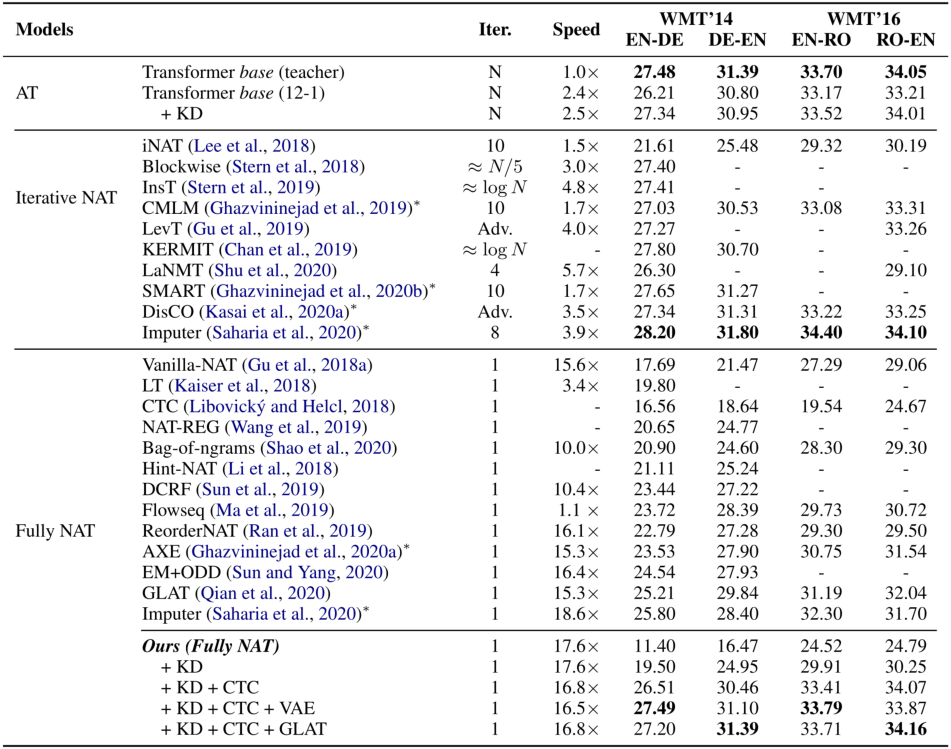
\includegraphics[width=0.9\linewidth]{./figure/Table2.pdf}
\end{center}
\end{frame}

\begin{frame}[label={sec:org7866e4c}]{Results: WMT20 JA \(\rightarrow\) DE}
\begin{center}
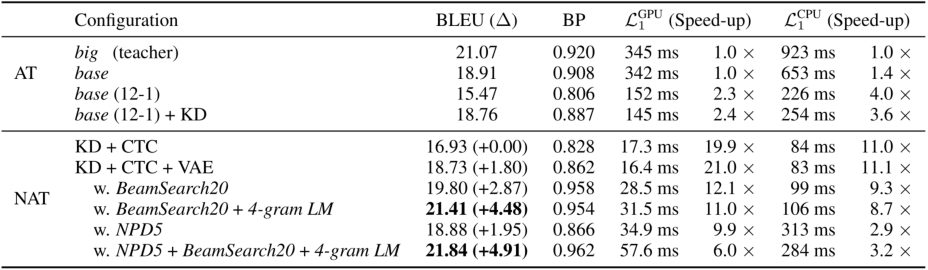
\includegraphics[width=\linewidth]{./figure/Table3.pdf}
\end{center}
\end{frame}

\begin{frame}[label={sec:org1037328}]{Quality v.s. Latency}
\begin{center}
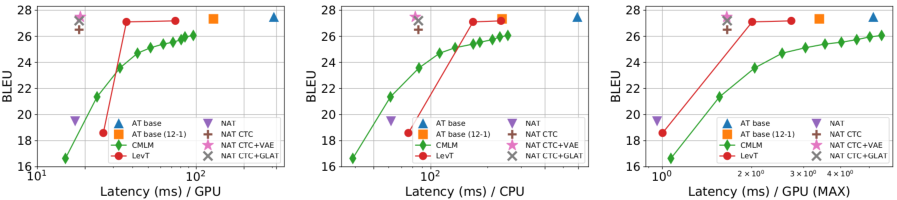
\includegraphics[width=\linewidth]{./figure/Figure4.pdf}
\end{center}
\end{frame}

\begin{frame}[label={sec:orgece0719}]{Ablation Study (on WMT14 EN \(\rightarrow\) DE)}
\begin{center}
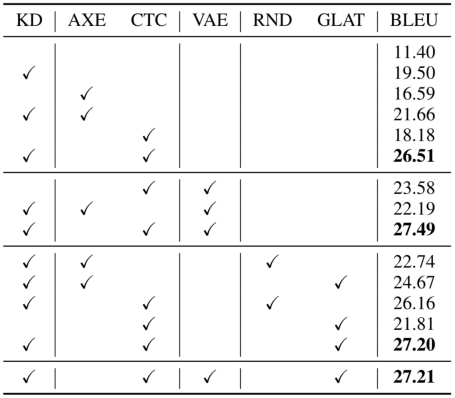
\includegraphics[width=0.7\linewidth]{./figure/Table4.pdf}
\end{center}
\end{frame}

\begin{frame}[label={sec:org048f385}]{Ablation Study (on WMT14 EN \(\rightarrow\) DE)}
\begin{center}
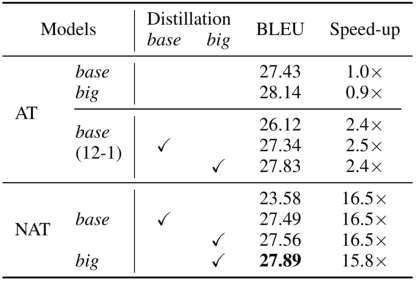
\includegraphics[width=0.7\linewidth]{./figure/Table5.pdf}
\end{center}
\end{frame}

\begin{frame}[label={sec:org84ef173}]{Upsampling Ratio ( \(\lambda\) ) for CTC Loss}
\begin{center}
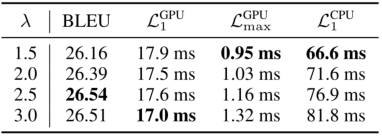
\includegraphics[width=0.7\linewidth]{./figure/Table6.pdf}
\end{center}
\end{frame}

\begin{frame}[label={sec:org320b040}]{Conclusion}
\begin{block}{fully NAT の性能が AT に追い付いた}
\begin{itemize}
\item 4 つの \textit{dependency reduction} によって SOTA な fully NAT モデルを設計
\begin{itemize}
\item Data: Knowledge Distillation
\item Model: Latent Variables
\item Loss Function: Latent Alignments
\item Learning: Glancing Targets
\end{itemize}
\end{itemize}
\end{block}
\end{frame}
\end{document}